
\begin{figure}[H]
    \centering
    \caption{Gradiente Descendente.}
    \label{fig:gradiente_desc}
    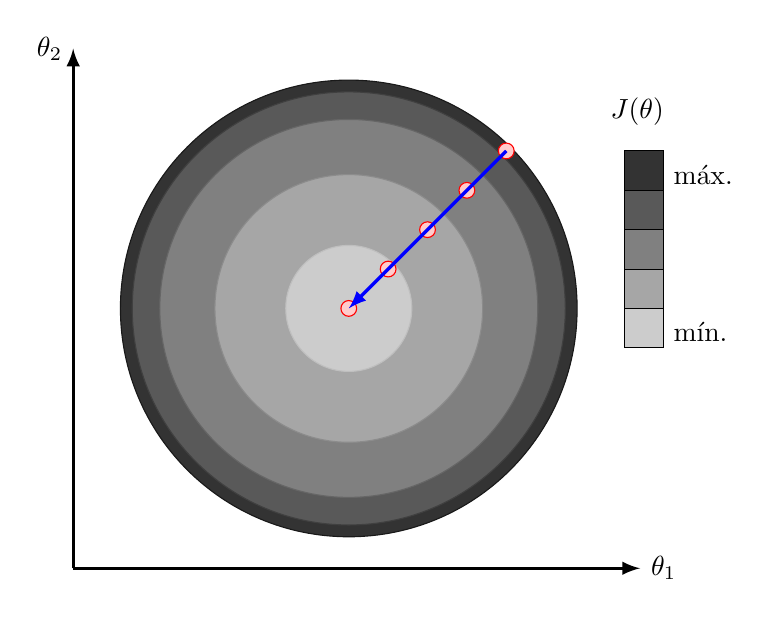
\begin{tikzpicture}
        % Círculos
        \filldraw[color=black!90, fill=black!80](-1,0) circle (2.9);
        \filldraw[color=black!75, fill=black!65](-1,0) circle (2.75);
        \filldraw[color=black!60, fill=black!50](-1,0) circle (2.4);
        \filldraw[color=black!45, fill=black!35](-1,0) circle (1.7);
        \filldraw[color=black!25, fill=black!20](-1,0) circle (0.8);
        
        % Pontos
        \foreach \i in {0, 0.5, 1, 1.5, 2}
        \draw[color=red, fill=red!20] (\i-1,\i) circle (0.1);
        
        % Seta
        \draw[-latex, color=blue, very thick] (1,2)--(-1,0);
        
        % Eixos
        \draw[-latex, color=black, very thick] (-4.5,-3.3)--(2.7,-3.3) node[right]{$\theta_1$};
        \draw[-latex, color=black, very thick] (-4.5,-3.3)--(-4.5,3.3) node[left]{$\theta_2$};
        
        % Legenda
        \draw (2.2, 2.5) node[right]{$J(\bm{\theta})$};
        \draw (3, 1.7) node[right]{máx.};
        \draw (3, -0.3) node[right]{mín.};
        
        % Degradê
        \draw[fill=black!80] (3, 2) rectangle (2.5, 1.5);
        \draw[fill=black!65] (3, 1.5) rectangle (2.5, 1);
        \draw[fill=black!50] (3, 1) rectangle (2.5, 0.5);
        \draw[fill=black!35] (3, 0.5) rectangle (2.5, 0);
        \draw[fill=black!20] (3, 0) rectangle (2.5, -0.5);
    \end{tikzpicture}
    \caption*{\small Fonte: Elaboração própria.}
\end{figure}
